\chapter{Theory and methods}
\label{chapter:theory}
\textit{\textbf{Add overview here}} \\
This chapter covers the theory behind light and particle interactions, 
and how the exact theory varies for differently sized particles. After 
that we show how this can be applied to existing diffusion models to 
accurately simulate the behaviour of a particle within the vicinity of 
an optical trap. Lastly, we highlight the techniques utilised in 
experiments to both calibrate and characterise an optical trap based 
on our understanding of the trap. 

%%%%%%%%%%%%%%%%%%%%%%%%%%%%%%%%%%%%%%%%%%%%%%%%%%%%%%%%%%%%%%%%%%%%%%%%%%%%%%%%%%%%%%%%%%%%%%%%%%%%%%%%%%%%%%%%%%%%%%%%%%%%%%%%%%%%%%%%%%%%%%%%%%%%%%%%%%%%
\section{Electromagnetism and optical tweezing}

Proper understanding of optical tweezing requires a description
of how the trapped particle interacts with the laser. From an
electromagnetism perspective the laser creates a spatially and 
temporally coherent electric field that scatters light when 
passing though a medium. The laws governing electric and magnetic 
fields are summarised most succinctly via the Maxwell equations. 
These four equations describe how the electric and magnetic fields 
behave and relate to one another. Any discussion of optical trapping 
is underpinned by the fact that in all cases the Maxwell equations 
must be satisfied. Macroscopic forms of the Maxwell equations are 
given below
\cite{Jackson_1975}:
\begin{align}
	\nabla \cdot \mathbf{D}
	&= \rho_f
	\\
	\nabla \cdot \mathbf{B}
	&= 0
	\\
	\nabla \times \mathbf{E}
	&= \frac{\partial \mathbf{B}}{\partial t}
	\\
	\nabla \times \mathbf{H}
	&= \mathbf{J}_f +\frac{\partial \mathbf{D}}{\partial t}  
\end{align}
where $\rho_f$ and $\mathbf{J}_f$ are the charge density and 
current caused by the presence of free charges in the medium, 
and $\mathbf{D}$ and $\mathbf{H}$ are the displacement and 
magnetising fields respectively. The latter two are defined by:
\begin{align}
	\mathbf{D} &= \epsilon\mathbf{E}+\mathbf{P} 
	\\ 
	\mathbf{H} &= \frac{1}{\mu}\mathbf{B}-\mathbf{M}
\end{align}
where $\mu$ is the vacuum permeability,, $\epsilon$ is the 
permittivity of free space, $\mathbf{P}$ is the polarization 
field and $\mathbf{M}$ is the magnetisation field, these 
fields arise due to the bound charges throughout the medium 
interacting with the EM field. 

The force exerted by an optical tweezer can be subdivided into 
the gradient and scattering components, for most modelling 
research this is how the force fields are reported. The gradient 
force is a conservative force brought about by the polarisation 
of dielectric materials which is directed towards the point of 
maximum intensity (for a simple Gaussian beam this would be at 
it's focal point) \cite{YasuhiroHarada1996}. Typically, optical 
tweezers will utilise a higher numerical aperture lens in order 
to increase the intensity, thus allowing for stronger gradient 
forces at the trade off of decreased trapping depth.

The scattering force arises from the motion of bound charges 
generating secondary scattering as they move through the 
electric field \cite{YasuhiroHarada1996}. Even if the particle
experiences no external forces the scattering force is still 
significant as the electric field oscillates, though for most
practical applications the time dependence is ignored. While 
some trapping arrangements can induce transverse scattering 
forces for simple spheres the scattering force is only 
significant in the direction of propagation \cite{Capitanio2002}.
In order to determine where a particle will remain at rest 
in an optical trap requires determining where the potential 
well formed by the gradient force is equal to the thermal 
energy of the system. 

%%%%%%%%%%%%%%%%%%%%%%%%%%%%%%%%%%%%%%%%%%%%%%%%%%%%%%%%%%%%%%%%%%%%%%%%%%%%%%%
\subsubsection{Harmonic Traps}
\label{sec:harmonic_traps}
When a sphere is located at the centre of a laser the gradient 
force will try to recentre the sphere if it is displaced. If 
the restoring force is proportional to the sphere's displacement 
this is referred to as a harmonic trap. The ratio of the restoring 
force to the displacement is called the trap stiffness (denoted 
by $\kappa$), and is an important characteristic of the trap. Fig.~\ref{fig:harmonic_trap} demonstrates an example case of the
force-displacement curve for a simple sphere in an optical trap. 
Laser power and numerical aperture are omitted as the exact shape 
is not of importance, only the linear region about the origin.
\begin{figure}[h!]
	\centering
	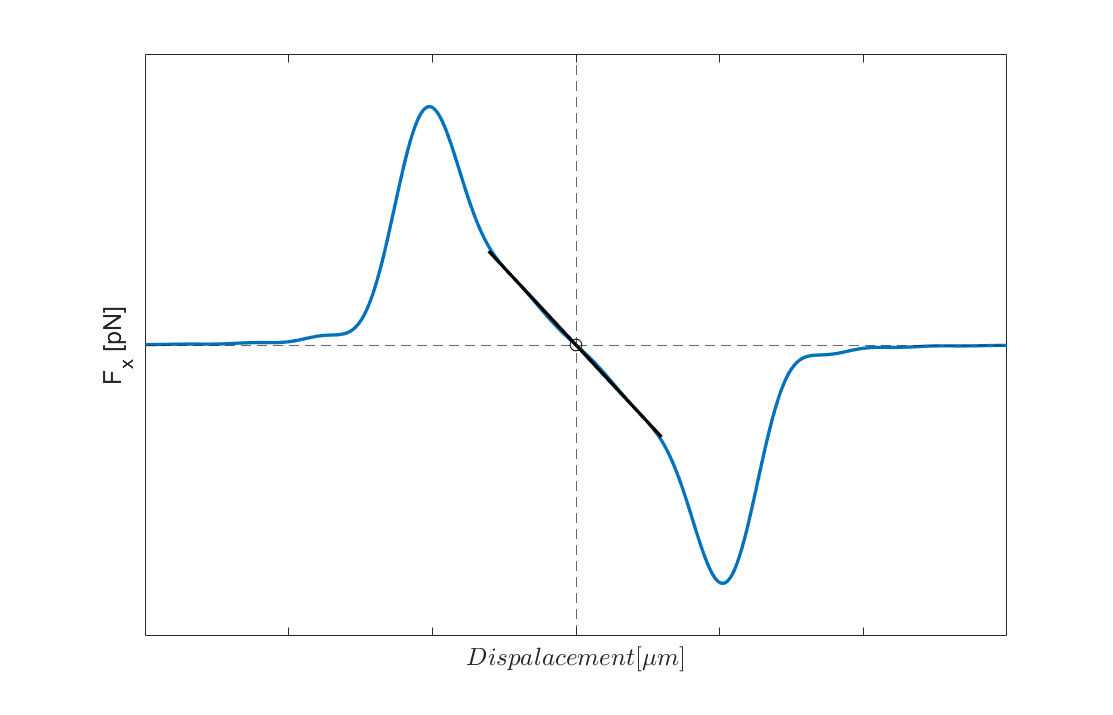
\includegraphics[width=1.1\linewidth]{sphere_force_curve.png}
	\caption{Example of a sphere's ($r=1\ \mu m$) force-displacement
		curve while moving along the x-axis, where $x=0$ is the 
		centre of the beam. The harmonic regime is highlight by the 
		linear fit given in black.}
	\label{fig:harmonic_trap}
\end{figure}

The strength of the optical trap is directly proportional to 
both the laser power and the contrast in refractive indices 
between the medium and the particle. Fully describing the 
optical forces is dependent on the ratio between the particle 
size ($a$) and the trapping wavelength ($\lambda$). The 
scattering theory that describes the optical force is dependent 
on this ratio.  
%%%%%%%%%%%%%%%%%%%%%%%%%%%%%%%%%%%%%%%%%%%%%%%%%%%%%%%%%%%%%%%%%%%%%%%%%%%%%%%
\section{Lornez-Mie Theory}

The Lorenz-Mie theory provides an exact solution to the Maxwell 
equations for the scattering caused by an isotropic sphere. This 
theory describes the scattered wave given off by a dielectric 
sphere when incident by a plane wave as a summation of partial 
spherical waves. For any wave equation the vector fields must 
solve the Helmholtz equation given by:
\begin{align}
	\nabla^2\mathbf{E} +k^2\mathbf{E} = 0
\end{align} 
where $k$ is the wave number of the electromagnetic radiation 
($k = \omega^2 \mu \epsilon/c^2$). This combined with the constraints of 
Maxwell's equations leaves very few exact solutions apart from 
spherical or planar waves. For a laser of arbitrary shape the 
electric field can be described as a summation of partial 
spherical waves multiplied by an expansion coefficient. Depending 
on the beam in question the expansion coefficients can be tailored
to match the desired beam shape. For a approximate Gaussian beam 
interacting with a sphere of radius $a$, the incident, internal, 
and scattered fields are given as \cite{RanhaNeves2019}: 
\begin{align}
	\label{eq:incident}
	{\bf E}_{\rm inc}({\bf r})
	&=
	E_0 \sum_{n}^\infty\sum_{m=-n}^n \left[
	a_{nm}{\bf M}_{nm}^{(1)}({\bf r})
	+ b_{nm}{\bf N}_{nm}^{(1)}({\bf r})\right]
	\\
	\label{eq:scattered}
	{\bf E}_{\rm scat}({\bf r})
	&=
	E_0 \sum_{n}^\infty \sum_{m=-n}^n\left[
	p_{nm}{\bf N}_{nm}^{(3)}({\bf r})+q_{nm}{\bf M}_{nm}^{(3)}({\bf r})
	\right] 
	\\
	\label{eq:internal}
	{\bf E}_{\rm int}({\bf r})
	&=
	{\bf E}_{\rm inc}({\bf r}) + {\bf E}_{\rm scat}({\bf r})
\end{align}

where $a_{nm}$, $b_{nm}$, $p_{nm}$, and $q_{nm}$
are the expansion coefficients of each of the fields, and ${\bf M}_
{nm}$ and ${\bf N}_{nm}$ are the magnetic and electric vector 
spherical harmonics respectively. The superscript denote whether 
the field is inward [(1)] or outward propagating [(3)]. By linearity 
of Maxwell's equations, its possible to relate the expansion 
coefficients of the scattered field directly to those of the incident 
field. As such we can write the scattering coefficients in terms of 
their incident components and the target's 'T-matrix'.
\begin{align}
	\label{eq:t_matrix}
	\begin{pmatrix}
		q_{mn} \\
		p_{mn} 
	\end{pmatrix}
	= \bold{T} 
	\begin{pmatrix}
		a_{mn} \\
		b_{mn}
	\end{pmatrix}
	= \begin{pmatrix}
		T_{11} & T_{12} \\
		T_{21} & T_{22}
	\end{pmatrix}
	\begin{pmatrix}
		a_{mn} \\
		b_{mn}
	\end{pmatrix}
\end{align}

Where the matrix \textbf{T} accounts for the targets shape, 
and refractive index. The $T$-matrix method can be easily 
applied to any solution of Maxwell's equations. In order to compute 
the optical force and torque applied to a given object one simply 
needs to know the momentum carried by the incident and scattered 
fields. So long as we know the expansion coefficients of the 
incident beam we can find the scattered beam coefficients via Eq.~\eqref{eq:t_matrix} to compute the force.

And the time averaged linear momentum carried by the scattered 
beam is given by:
\begin{equation}
	\label{eq:linear_momentum_out}
	\begin{split}
		\langle P_{z,\ out} \rangle
		&=
		-\frac{1}{4\pi k^2}\sum_{n,m} \left(\frac{m}{n(n+1)}\Im[p_{nm}q^*_{nm}] \right.
		\\ 
		&+\frac{1}{n+1}\left[\frac{n(n+2)(n-m+1)(n+m+1)}{(2n+1)(2n+3)} \right]^{1/2}
		\\
		& \left.\times\Im[q_{nm}q^*_{nm}+p_{nm}p^*_{n+1m}] \right)
	\end{split}
\end{equation}

Therefore the total force imparted to the trapped particle is thus:
\begin{align}
	\boldsymbol{F_z} =\frac{dP}{dt} = \langle P_{z,\ in}\rangle 
	-\langle P_{z,\ out}\rangle
	\label{eq:Fz}
\end{align}

\noindent
Where $a_{nm}, b_{nm}, p_{nm}, \& q_{nm}$ are the beam expansion 
coefficients used in \eqref{eq:incident} \& \eqref{eq:scattered}.
Similar expressions are shown in Sec.~\ref{sec:simulations} for 
calculating the optical torque. Lorenz-Mie theory can be applied 
to describe the scattering from any particle regardless of size.
Though as the size of the target particle changes - relative to 
the wavelength of light - the theory describing the electromagnetic 
fields are easier to approximate by alternative theories. When the 
particle radius is $\gg \lambda$ the optical force is best described 
by the Ray-Optics model. In the opposite case the target particle is 
better approximated as a single electric dipole as described by 
the Rayleigh approximation.  
%%%%%%%%%%%%%%%%%%%%%%%%%%%%%%%%%%%%%%%%%%%%%%%%%%%%%%%%%%%%%%%%%%%%%
\subsection{T-matrix Method}
The $T$-matrix method was first developed by Peter Waterman with 
his research into acoustic wave scattering \cite{Waterman1969}, 
this would later be extended to electromagnetic waves. Sometimes 
referred to as the extended boundary condition method (EBCM), the 
method replaces the scatterer with a series of surface currents 
over the targets surface. These currents are chosen so that the 
electromagnetic field outside is identical to the original problem 
\cite{Wriedt1998}. By expanding the harmonic functions one can 
derive the individual elements of \textbf{T} until a desired 
accuracy is achieved. One can either use the EBCM to compute the 
scattering for a fixed particle orientation and position. Or they
can evaluate the scattering for any particle orientation by 
computing its $T$-matrix. Because the T-matrix is based only 
on the properties of the scatterer it can be reused in 
calculations regardless of the incident field in question.

For this project we utilised an extension of the EBCM known as 
multi-sphere $T$-matrix method (\textit{mstm}) developed by 
Mackowski \cite{Mackowski2011}. Where Lorenz-Mie Theory centres
the spherical harmonics expansion about the sphere's origin it
often struggles to adjust the expansion to any arbitrary origin.
\textit{mstm} utilises an addition theorem to translate the 
individual spherical expansions from the centres of each 
individual sphere to a preset target origin. \textit{mstm}'s 
primary function is to compute the averaged scattering from 
large spherical aggregates, but for our purposes it can be
also utilised to compute $T$ matrices for arbitrary shaped
spherical aggregates.

The $T$-matrix method is exceptionally useful for computing the 
scattering from any arbitrary spherical aggregate. However, the 
$T$-matrix method by itself can be computationally taxing as the 
number of spheres increases \cite{Mackowski2011}. While it is 
possible to solve for the full electromagnetic field for the 
entire cluster this is only applicable for a single orientation 
and can be even slower for large aggregates \cite{Mackowski1996, 
	Xu1995}. The benefit of \textit{mstm} is that the major scattering 
properties (scattering and extinction cross sections, scattering 
matrices, etc) can all be computed both for single orientations, 
or averaged over multiple orientations to determine the average 
scattering from the target particle. 

%%%%%%%%%%%%%%%%%%%%%%%%%%%%%%%%%%%%%%%%%%%%%%%%%%%%%%%%%%%%%%%%%%%%%%%%%%%%%%
\subsection{Discrete Dipole Approximation}
The discrete dipole approximation (DDA) is a general method that 
can be applied to the scattering from particles of arbitrary 
composition and geometry. Developed by Purcell and Pennypacker 
\cite{Purcell1973}, the DDA method approximates the particle as 
being constructed of discrete dipoles. This is essentially an 
extension of the Rayleigh approximation, though in order to compute 
the optical force one now requires a full description of the electric 
field. Each dipole interacts with both the incident field and the 
scattered fields from every other dipole surrounding it. The 
resulting scattered field is identical to the scattered field 
produced by direct integration of Eq.~\eqref{eq:internal} 
throughout the full particle volume \cite{Goedecke1988}. The 
integral form for the total electric field inside a scatterer is 
given as \cite{Wriedt1998}:
\begin{align}
	\mathbf{E(r)} = \mathbf{E}_{inc}(r) + \sum^{N_d}_{i}\mathbf{E}_{scat,i} =  
	\mathbf{E}_{inc}(r) + \int_{V/V_0}d^3r\mathbf{\bar{G}(r,r')}
	\chi(\mathbf{r'})\mathbf{E(r')}
	\label{eq:DDA}
\end{align}

Where $\mathbf{\bar{G}}$ is the Greens dyadic function of free space, 
which defines the impulse response between two separate dipoles; and 
$\chi$ is the susceptibility of the medium, which describes the 
degree of polarisation of the medium in the presence of an electric 
field. One of the primary advantages of DDA over the T-matrix method 
is that the composition of the target can be changed freely. When 
comparing different computational scattering methods, the EBCM was 
found to be better suited for simulating the scattering of symmetric
targets as the EBCM can use the target's symmetry to speed up 
calculations \cite{Wriedt1998}. But when dealing with inhomogeneous 
media DDA is more efficient compared to EBCM. 

The DDA method can be used to derive the target's $T$-matrix. After
generating the far field expansion of the electric field (Eq.~
\eqref{eq:DDA}), the vector spherical expansion far field 
(Eq.~\eqref{eq:scattered}) can be matched to it. Solving for the 
expansion coefficients $p_{nm}$, and $q_{nm}$ allows one to construct
the T-matrix of the target. 
\newpage

%%%%%%%%%%%%%%%%%%%%%%%%%%%%%%%%%%%%%%%%%%%%%%%%%%%%%%%%%%%%%%%%%%%%%%%%%%%%%%
\section{Ray-Optics Regime}

The Ray-Optics model is the simplest to understand, this theory models 
the electromagnetic field as a collection of individual 'rays' that 
propagate and are refracted according to Snell's Law. Based on the 
change in direction momentum is transferred to the target particle; 
with rays closest to the centre of the beam having greater intensity 
than those rays at the very edge of the beam. Consider a particle 
struck by two rays in a Gaussian beam, one coming close to the centre, 
and the other ray coming from the edge. As each ray is refracted by 
the target sphere a force is imparted onto it, the total force 
imparted is given by:
\begin{align}
	F_i = Q_i\frac{\Delta n P_i}{c}
\end{align}

\noindent 
where $Q_i$ is the trapping efficiency, $\Delta n$ is the difference
in refractive indices between the solution and the target particle,
and $P_i$ is the power of the individual ray. The net force can be 
subdivided into its gradient and scattering components, where the latter
directs the particle to the centre of the beam, and the former acts on 
the particle in the direction of beam propagation. For a beam with a
Gaussian intensity distribution $P_i$ will fall off as you move from
the centre of the beam. The ray optics model is ideal when dealing 
with larger particles whose diameter far exceed the wavelength of light
being scattered. While it can be useful in predicting the forces 
experienced by said particle's it does not fully capture the behaviour
of light when considering interference between different rays. And 
as such no information is learned about the scattered field.

%%%%%%%%%%%%%%%%%%%%%%%%%%%%%%%%%%%%%%%%%%%%%%%%%%%%%%%%%%%%%%%%%%%%%%%%%%%%%%%%
\section{Rayleigh Scattering}

The Rayleigh approximation is for describing a particle when 
the particle radius is $\ll \lambda$. The underlying theory 
is that a dielectric sphere can be treated as a dipole while 
in the presence of the electromagnetic field. In which case 
the scattering force is given simply by the scattering of 
the induced dipole, and the gradient force is due to the 
Lorentz force \cite{Gordon1973}. The gradient forces in the 
principle Cartesian axis are described by Harada et al \cite{YasuhiroHarada1996} in MKS units as a restorative 
rectangular force field:
\begin{align}
  F_{grad,x}
  &=-\hat{x} \frac{2\pi n_2 a^3}{c}
    \left(\frac{m^2-1}{m^2+2}\right) \frac{4\tilde{x}/w_0}{1+(2\tilde{z})^2} \times I(r)
  \label{eq:Rayleigh_start}\\
  F_{grad,y}
  &=-\hat{y} \frac{2\pi n_2 a^3}{c}
    \left(\frac{m^2-1}{m^2+2}\right) \frac{4\tilde{y}/w_0}{1+(2\tilde{z})^2} \times I(r)
  \\
  F_{grad,z}
  &=-\hat{z} \frac{2\pi n_2 a^3}{c}
    \left(\frac{m^2-1}{m^2+2}\right) \frac{4\tilde{z}/w_0}{1+(2\tilde{z})^2}
    \nonumber \times I(r)
  \\ 
  & \times \left[1-\frac{2(\tilde{x}^2+\tilde{y}^2)}{1+(2\tilde{z})^2} \right]
  \\
  \label{eq:Rayleigh_end}
\end{align}
where, for a approximate Gaussian beam the intensity $I(r)$ 
close to the beam focus can be calculated as such.
\begin{align}
  \nonumber
	I(r) &= \left(\frac{2P}{\pi w_0^2}\right) \frac{1}{1+(2\tilde{z}^2)} 
	\exp \left[ - \frac{2(\tilde{x}^2+\tilde{y}^2)}{1+(2\tilde{z})^2} \right]
\end{align}

\noindent
Where $m$ is the relative refractive index ($n_1/n_2$), $n_2$ is 
the particle's refractive index, $\omega_0$ is the beam waist, 
$a$ is the radius of the particle, and $\tilde{x}, \tilde{y}, 
\tilde{z}$ are simply the $x, y, z$ coordinates but scaled by the 
beam radius. The scattering force however, is dependent on the 
effective scattering cross-sectional area. 
\begin{align}
  F_{\rm scat}
  &= \hat{z} \left(\frac{n_2}{2}\right) C_{pr} I(r) \\
  \text{where:} \nonumber \\
  C_{pr} &= \frac{8}{3} \pi (ka)^4 a^2 \left(\frac{m^2-1}{m^2+2}\right)^2
\end{align}

There is a clear difference between Eq.~\eqref{eq:Rayleigh_start}-
\eqref{eq:Rayleigh_end} and Eq.~\eqref{eq:linear_momentum_in}- \eqref{eq:Fz}, namely that the Rayleigh regime is not concerned with 
the state of the scattered field. This is because if the particle 
is approximated by a point dipole we can ignore the momentum 
transfer calculation and simply compute the Lorenz force for a 
dipole in an electric field. While not important for optical force calculation higher complexity scattering problems can be simplified 
by subdividing the particle into discrete dipoles (see Sec~\ref{sec:scattering}), in which case the scattered field is now significant. As the target particle gets larger this approximation 
fails to accurately describe the trapping force \cite{Li2021}. For 
larger particles the optical force and scattering is better described 
via the Lorenz-Mie theory. 

%%%%%%%%%%%%%%%%%%%%%%%%%%%%%%%%%%%%%%%%%%%%%%%%%%%%%%%%%%%%%%%%%%%%%%%%%%%%%%
%%%%%%%%%%%%%%%%%%%%%%%%%%%%%%%%%%%%%%%%%%%%%%%%%%%%%%%%%%%%%%%%%%%%%%%%%%%%%%
%%%%%%%%%%%%%%%%%%%%%%%%%%%%%%%%%%%%%%%%%%%%%%%%%%%%%%%%%%%%%%%%%%%%%%%%%%%%%%
\section{Describing the trajectory of a trapped particle}
While describing the optical forces is sufficient for 
theoretical characterisation of an optical trap, in an 
experimental setting the observed motion is not as 
simple. As such it is often far simpler to 
characterise the optical trap by recording the particle's
trajectory (see \ref{sec:position_detection} for 
specifics regarding the equipment), and then fitting it 
to our presumed description of the beam. The trajectory 
is easily understood if we understand the particle's 
diffusive behaviour.

\subsection{Langevin Equation}
Describing any microscopic motion requires an understanding 
of a molecules diffusive behaviour, for the case of optical 
tweezers the most complete model of diffusion is the Langevin 
equation. Models such as the Fickian, and Einstein derivations 
are sufficient for macroscopic behaviours but the Langevin 
model better describes the microscopic characteristics of 
any diffusive behaviour.
 
The Fickian model describes the net flux of solute molecules 
into a finite volume of fluid being proportional to the 
density gradient $\delta\rho(u,t)/\delta u$ \cite{Gillespie2012}. 
It assumes that the solute molecules do not collide with one 
another or with molecules in the solution; overall, the Fickian 
model is used to describe how solute molecules disperse over 
long periods of time. It does not provide any insight into 
the forces acting on individual molecules, nor does it prove 
particularly useful over smaller time scales. Whereas the Langevin 
model captures the physical interactions between an individual 
molecule and the surrounding fluid over a wide range of time 
scales.

The Einstein model of diffusion expands upon the Fickian model 
by considering the collisions between individual molecules. If 
we consider a single particle suspended in a solution it will 
experience multiple collisions with other molecules 
\cite{Gillespie2012a} over a given time interval $\delta t$. 
Applying statistical analysis to an observed trajectory allows
one to make measurements of a particle's diffusive behaviour 
within a fluid. Where it begins to falter is when we consider 
bringing $\delta t$ to $0$; in this scenario the molecule 
experiences not many but only individual collisions. The 
Einstein model does not consider the inertia of the molecule 
in question and so for very short time frames the model 
implies that the molecule's velocity changes instantly after 
each collision \cite{Gillespie2012a, Gillespie2012b}. 
Furthermore, the kinetic energy of each collision is not 
limited by the thermal energy of the system, meaning that 
using the Einstein model to predict a particle's trajectory 
to an finite degree of accuracy implies that the particle 
has infinite kinetic energy \cite{Gillespie2012b}. This 
failure to describe motion over smaller time frames is 
addressed in the Langevin model by accounting for the fluid 
drag of the system, where any sudden change in velocity must 
result in a proportionally opposed drag force \cite{Gillespie2012c}. 

The Langevin model of diffusion assumes that the net force on 
a particular particle is described fully by these individual 
collisions \cite{Gillespie2012c}. Unlike the Fickian model it 
provides a full description of the interactions between the 
target molecule and the surrounding fluid; while also being 
able to describe its motion over any time scale, unlike the 
Einstein model. The standard form of the Langevin model for 
a particle undergoing Brownian motion is given as:
\begin{align}
	m\frac{dv}{dt} + \gamma_0 v + F(t) = W(t)
\end{align}

Where the first term accounts for inertial forces, the second 
term accounts for friction forces which counteract the particles 
current motion ($\gamma_0$ is the friction coefficient), and 
the final term accounts for the random Brownian force. The 
$F(t)$ is there for convention which accounts for any external 
forces acting on the particle. These three terms are equal to 
the random Brownian motion of the surrounding fluid. We can 
say that the noise term $W(t)$ has a normal distribution, 
being scaled by the thermal energy of the system, with a 
correlation function of:
\begin{align}
	&W(t) = \sqrt{2k_BT\gamma_0}\eta(t) \\
	&\langle W_i(t)W_j(t')\rangle = 2k_BT\gamma_0\delta(t-t')
\end{align}

The Langevin model can be extrapolated to describe the diffusive 
behaviour of an overall system, but for this project we can 
instead consider the behaviour of a singular particle with a diffusion 
tensor $D$ suspended in a viscous fluid and spacially localised 
by an optical potential with trap strength $\kappa$. Assuming the 
only external force acting on our particle is the laser, the net 
force should be exactly equal to force of the stochastic collisions 
due to the fluids thermal energy. If we focus our analysis when 
the particle is stably trapped and assume that the trap is harmonic, 
we can model the trapping force as a Hookean spring ($F(t) \approx 
\kappa x(t)$). The full Langevin equation for an optically trapped 
particle is therefore given as:
\begin{align}
	\label{eq:langevin}
	m\frac{\delta^2x(t)}{\delta t^2} + \gamma_0 \frac{\delta x(t)}{\delta t} + \kappa_x x(t) = \sqrt{2k_BT}\eta(t)
\end{align}

Eq.~\eqref{eq:langevin} provides an accurate description of strongly 
trapped particles. Despite this the analytical solution of the 
Langevin equation requires integration of the noise term making 
it difficult to simulate the trajectory of a given particle 
\cite{Volpe2013}. Instead, it is often far easier to solve the 
equation numerically and use the analytical solution to calibrate 
and extract information about the particle and fluid, and how the 
two interact with the optical trap. Solving the Langevin equation
numerically is far easier when considering small time steps.

\subsection{Finite Difference}
The Finite Difference approach involves discretizing the time and 
spatial elements in order to approximate the higher order terms. 
If we assume that $x(t)$ is differentiable to n (we can find its 
$n^{th}$ derivative) then we can use the Taylor series expansion 
to get:
\begin{align}
	x(t+\Delta t) = x(t)+\frac{x'(t)}{1!}\Delta t + \frac{x^2(t)}{2!}\Delta t^2+...+\frac{x^n(t)}{n!}\Delta t^n+R_n(x(t))	
\end{align}

Where $R_n(x(t))$ is the remainder term between the Taylor 
expansion to term n and the actual expression. If we limit our 
approach to the first derivative only, we find that for 
sufficiently small values of $R_1$ the velocity and acceleration 
can be approximated as:
\begin{align}
	x'(t) &\approx \frac{x(t+\Delta t)-x(t)}{\Delta t}
	\\
	x^{''}(t) &\approx \frac{x'(t+\Delta t)-x'(t)}{\Delta t} = \frac{x(t)-2x(t+\Delta t)+x(t+2\Delta t)}{\Delta t^2}
\end{align}

By reversing the time step (i.e. use $-\Delta t$) to approximate 
the velocity and acceleration based on the previous time steps, 
we can discretise the position by taking finitely small  time 
steps (i.e. $x(t) = x_i,\ x(t-\Delta t) = x_{i-1}$). The same 
cannot be done for noise, as no information is known about $W(t)$ 
at any time. We can instead say that the velocity of a Brownian 
particle should approximate our noise as a random walk, where at 
each new time step, the position changes randomly within a given 
range. Constricting the variance to $\sqrt{2D}/\Delta t$ allows 
us to represent the noise using the finite-difference approach as:
\begin{align}
	m\frac{x_i-2x_{i-1}+x_{i-2}}{\Delta t^2} = -\gamma\frac{x_i-x_{i-1}}{\Delta t}+\sqrt{2k_BT\gamma}\frac{w_i}{\sqrt{\Delta t}}
\end{align}

Where $w_i$ is a random real number between -1 and 1, we can say 
that it is normally distributed around 0 for simulation purposes. 
We can rearrange this for $x_i$ to approximate the Brownian motion 
of a particle (setting $x_0=0$), where the characteristic time is 
$\tau = m/\gamma$. Now in the case of an optical trap, the 
restoration time scale is given by $\tau_{OT}=\kappa_x/\gamma$ 
which for strongly trapped particles is far greater than the 
characteristic time. As such we can neglect the particle's inertia 
which allows the motion of an optically trapped particle to be written 
as:
\begin{align}
	\label{eq:sim_langevin}
	x_i = x_{i-1} - \tau_{OT}\ x_{i-1}\Delta t + \sqrt{2D\Delta t}\ w_i
\end{align} 

This result can be generalised for a 3-dimensional description of 
an optically trapped particle, where each Cartesian direction has 
its own unique characteristic restoration time. We see from the 
result that trajectory is dependent on only a handful of factors, 
the trap stiffness $\kappa_x$, the fluid viscosity $\gamma$, and 
the thermal energy of the system $k_BT$ (with the latter two being 
related by Einstein's formulation of the diffusion coefficient $D = k_BT/\gamma$). Therefore, by calculating these parameters to a high 
degree of precision allows one to get a precise description of the 
forces experienced by a target particle, which in the past has been 
used for highly accurate force transduction \cite{BergSoerensen2004, Smith2003}.
\begin{SCfigure}[][h!]
	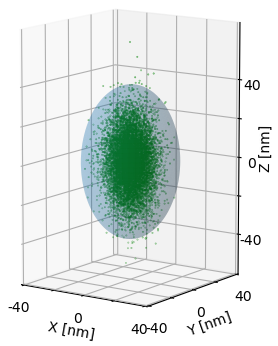
\includegraphics[height=0.68\linewidth]{finite_differences.png}
	\caption{\rule{0ex}{20ex}Example trajectory created using Finite 
		Differences method for a $2\mu m$ diameter sphere. Trap 
		stiffness's were estimated using \textit{ott} at $\kappa_x = 
		\kappa_y = -100\ pN/\mu m$ and $\kappa_z = -25\ pN/\mu m$. 
		The particle's motion can be localised around the shaded ellipsoid.}
\end{SCfigure}

%%%%%%%%%%%%%%%%%%%%%%%%%%%%%%%%%%%%%%%%%%%%%%%%%%%%%%%%%%%%%%%%%%%%%%%%%%%%%%
%%%%%%%%%%%%%%%%%%%%%%%%%%%%%%%%%%%%%%%%%%%%%%%%%%%%%%%%%%%%%%%%%%%%%%%%%%%%%%
\section{Simulation of spherical aggregates}
\label{sec:simulations}
Later chapters cover the dynamics of spherical aggregates and anisotropic 
scatterers, these subjects are particularly difficult to characterise 
using conventional calibration techniques \cite{Li2008, Yogesha2011PreciseCO}. 
As an example consider a symmetric dimer as a paradigmatic aggregate; 
if we consider the Langevin equation for such a aggregate within an optical 
trap we have:
\begin{align}
	\frac{{d}\vec{r}(t)}{{dt}} = \frac{\vec{\kappa}_x}{\gamma}\vec{r}(t) + 
	\sqrt{2\vec{D}_x}\eta(t)
\end{align}

Where $x(t)$ is replaced with $\vec{r}(t)$ to signify that the translational 
motion is generalised to a 3 dimensional case. Here we omit the inertia term 
as the restoration time of the optical trap is far greater than the characteristic time of the particle ($\kappa/\gamma \gg m/\gamma$). Now, the dimer is undergoing random rotational motion in addition to its Brownian 
translational motion the first term on the right hand side is no longer 
purely a function of the dimer's position but also of its orientation. 
The rotational form of the Langevin equation for a dipole within an external 
potential is given as \cite{Mazo2008}:
\begin{align}
	\frac{{d}\vec{u}(t)}{{dt}}
	=
	\frac{\mu}{\gamma_R}\left[\vec{u}(t)\times E(t)\right]\times \vec{u}(t)
	+ \sqrt{2k_BT\vec{D}_R}\lambda(t)\times \vec{u}(t)
\end{align}

Where $\vec{u}(t)$ is the unit vector aligned along the centres of 
the two spheres, $\mu$ is its dipole moment, and $\gamma_R$ is the 
rotational friction coefficient which is given as $\gamma_R = 8\pi
\eta r^3$ for a sphere. If we assume that over the course of a 
trajectory the dimer has a 'equilibrium' orientation in which the 
optical torque is minimised we can say that the first right hand 
term can be replaced with $\vec{\kappa}_u(\vec{r}(t))$ to represent
a harmonic potential due to the torque. $\lambda(t)$ is the Brownian 
rotations from the surrounding fluid, like in the translational case 
the Brownian rotations are normally distributed and are also uncorrelated 
so that:
\begin{align}
	\left<\lambda(t)\lambda(t')\right> = \delta_{ij}\delta(t-t')
\end{align}

For an asymmetric scatterer whose radius is comparable to that of the 
electric field's wavelength we now have a system of simultaneous equations:
\begin{align}
	\label{eq:full_langevin}
	\frac{{d}\vec{r}(t)}{{dt}}
	&=
	\frac{\vec{\kappa}_x(\vec{u}(t))}{\gamma}\vec{r}(t) + \sqrt{2k_BT\vec{D}}\eta(t)
	\\
	\frac{{d}\vec{u}(t)}{{dt}}
	&=
	\frac{\vec{\kappa}_u(\vec{r}(t))}{\gamma_R}\times \vec{u}(t)
	+ \sqrt{2k_BT\vec{D}_R}\lambda(t)\times \vec{u}(t)
\end{align}

Fortunately, we do not need to solve these directly as the latter two
random variables can be easily approximated if the thermal energy of
the system is known, and the rate of change can be assumed as linear if
we take a sufficiently small time step that $\Delta t~\ll~\kappa_x/\gamma 
\ \& \ \Delta t \ll \kappa_u/\gamma_R$. In doing so we now only need 
to compute the optical force and torque applied to the dimer. 

Using a  MATLAB package called \textit{Optical Tweezer Toolbox} 
or \textit{ott} \cite{Nieminen2007} we can compute the beam 
shape coefficients ($a_{nm}$ \& $b_{nm}$) for any desired beam 
type. Using the results from \cite{Farsund1996} we can then 
compute both the optical force and torque using the beam 
coefficients and the scattering coefficients ($q_{nm}$ \& $p_{nm}$) 
which are found by calculating the dimer's $T$-matrix via \textit{mstm} 
\cite{Mackowski2011} and then using \eqref{eq:t_matrix}. The 
total force in along the z-direction and the total torque about 
the z-axis are provided:
\begin{equation}
	\label{eq:optical_force}
	\begin{split}
		\bold{F_z}
		&=
		-\frac{1}{4\pi k^2}\sum_{n,m} \left(\frac{m}{n(n+1)}\Im[a_{nm}b^*_{nm}-p_{nm}q^*_{nm}] \right.
		\\ 
		&+\frac{1}{n+1}\left[\frac{n(n+2)(n-m+1)(n+m+1)}{(2n+1)(2n+3)} \right]^{1/2}
		\\
		& \left.\times\Im[b_{nm}b^*_{nm}+a_{nm}a^*_{n+1m}-q_{nm}q^*_{nm}+p_{nm}p^*_{n+1m}] \right)
	\end{split}
\end{equation}
\begin{equation}
	\begin{split}
		\bold{T_z}
		&=
		-\frac{1}{8\pi k^3}\sum_{n,m} \left(\frac{m}{n(n+1)}[|a_{nm}|^2+|b_{nm}|^2-|p_{nm}|^2-|q_{nm}|^2] \right.
		\\ 
		&+\frac{2}{n+1}\left[\frac{n(n+2)(n-m+1)(n+m+1)}{(2n+1)(2n+3)} \right]^{1/2}
		\\
		& \left.\times\Re[b_{nm}a^*_{nm}+a_{nm}b^*_{n+1m}-p_{nm}q^*_{nm}+q_{nm}p^*_{n+1m}] \right)
	\end{split}
\end{equation}

where $a_{nm}$, $b_{nm}$, $p_{nm}$, and $q_{nm}$ are the beam 
coefficients of the incident and scattered fields respectively. 
We can get the $x$ and $y$ force and torque components in a 
similar form by applying a simple rotation transformation. With 
the optical forces and torques computed all that remains is to 
compute the Brownian forces and torques which are constrained 
by the relation.
\begin{align}
	\langle q_iq_j\rangle =2D_{ij}\Delta t
\end{align}

Vigilante et al compiled together a python package that combines 
both \textit{ott} and \textit{mstm} to simulate the behaviour of 
spherical aggregates within a predefined optical trap 
\cite{Vigilante2020}. Now \textit{ott} does have inbuilt $T$-matrix 
modules that can be used to model the scattering from different 
shaped particles; however, for aggregates of spheres the resultant 
force is nonsensical (see Chapter 4 for further details). As such 
we rely on the \textit{mstm} for simulating dimers.  
%%%%%%%%%%%%%%%%%%%%%%%%%%%%%%%%%%%%%%%%%%%%%%%%%%%%%%%%%%%%%%%%%%%%%%%%%%%%
%%%%%%%%%%%%%%%%%%%%%%%%%%%%%%%%%%%%%%%%%%%%%%%%%%%%%%%%%%%%%%%%%%%%%%%%%%%%

\section{Calibration Techniques}
\label{sec:calibration_techniques}
There are several approaches for calibrating and characterizing 
the optical trap, each approach has its drawbacks and benefits 
so each option should be chosen based on what elements want to 
be characterized. The basis for each of these methods stems from 
the analytical solution of the Langevin equation:
\begin{align}
	\label{eq:anylitical_lang}
	x(t) = x(0)e^{-t/\tau_{OT}}+\sqrt{2D}\int^t_0dsW_x(s)e^{-(t-s)/\tau_{OT}}
\end{align}

Positional data is often acquired in an experimental setting 
either using image analysis or photodiodes to infer the particles 
position relative tothe beam focus. The former is often used in 
cases when precision is not a key concern, as often a standard 
CCD camera will have limited spacial and temporal resolution. 
The latter method often requires the use of a quadrant photo 
diode(QPD), the data provided by the QPD will often need to be 
converted to physical units to compute the force directly - see Eq.~\eqref{eq:conversion_factor}.

\subsection{Beam shapes}
A quick aside is necessary prior to the discussion 
of calibration techniques, namely on the assumption 
of the beams shape. It has been previously mentioned 
that the focused beam can be approximated as a 
Gaussian beam, what this implies is that the beam has 
a circularly symmetrical intensity profile that can be
described by the Gaussian function. There are alternative 
beam formations that also preserve the circularly 
symmetric profile, such as Bessel beams that have an 
intensity profile that is described by the Bessel 
function. 
\begin{figure}
	\centering
	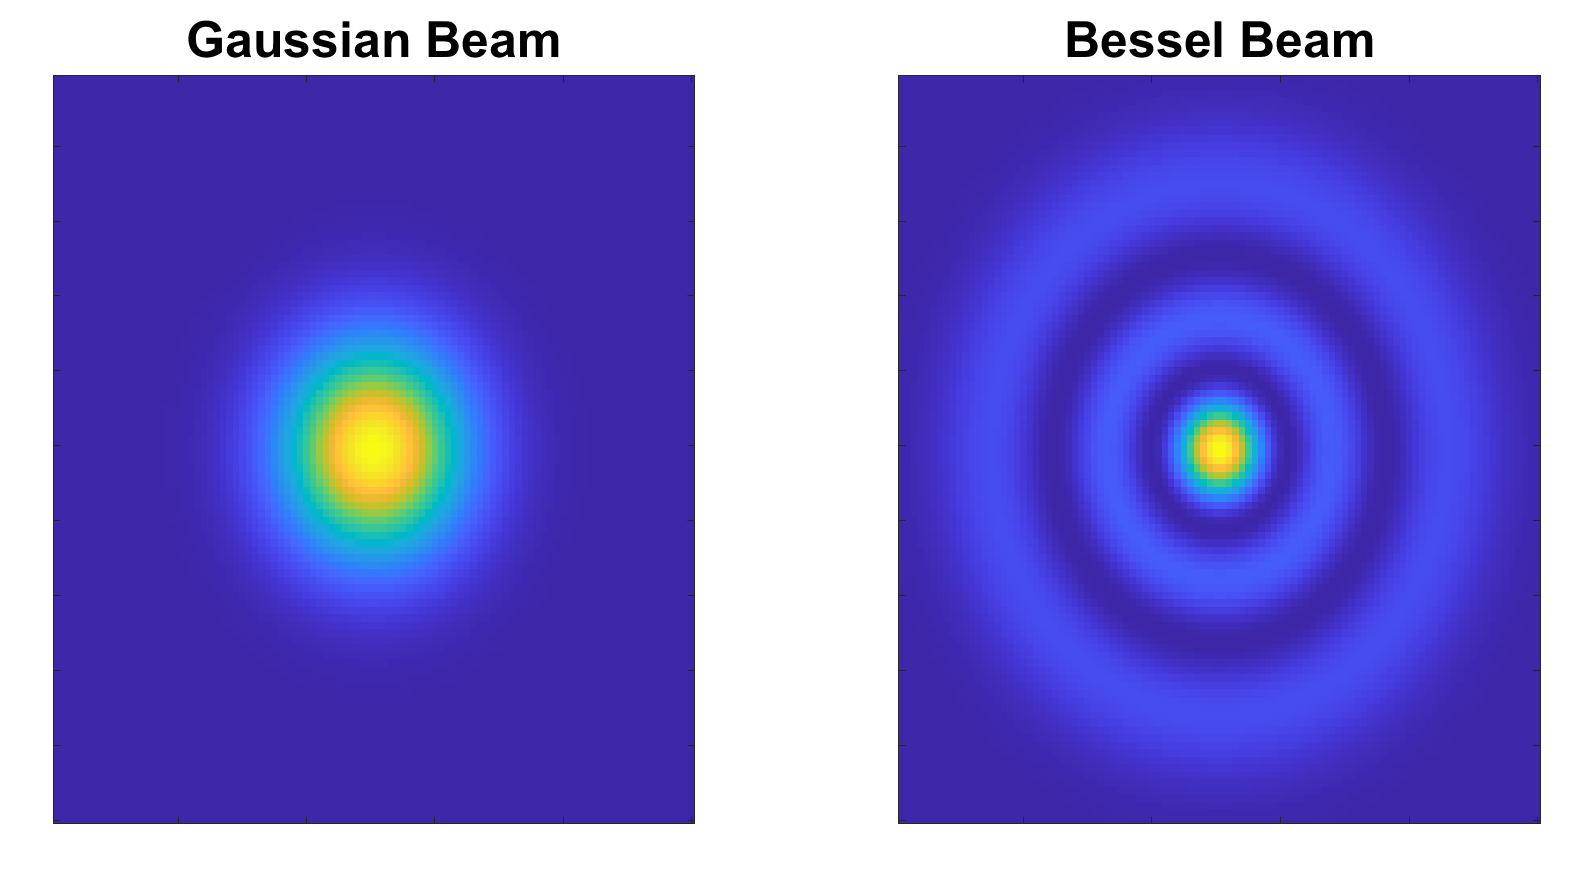
\includegraphics[width=\linewidth]{Gaussian_Bessel.png}
	\caption{Intensity distribution from a Gaussian and Bessel
	beam.}
\end{figure}

An idealised form of a Gaussian and Bessel beam would be 
unbounded, meaning the intensity of the electric field 
never goes to 0 - approaching it asymptomatically instead. 
This however breaks Maxwell's Equations (see Eq.
\eqref{eq:max_start} - \eqref{eq:max_end}), what this 
means is that in reality is that a true Gaussian or Bessel 
beam cannot exist, only a close approximation \cite{Gouesbet1988}. 
Due to the converging fields, a focused beam will experience 
fluctuations in its electric field that distort the intensity 
profile \cite{Lock1994}. This effect is insignificant 
for slowly converging beams but for trapping objectives 
used in optical tweezing there is a notable effect. 

When a Gaussian beam is linearly polarised and 
focused to a point the focal point will not be 
perfectly symmetrical but instead show some 
degree of ellipticity even if the initial beam 
itself is kept parallel. In practical terms this
means that regardless of the calibration 
technique used the trap stiffness along the x and
y axis will not be equal to one another. Proper
alignment can bring them close together and longer
data acquisition times can reduce the uncertainty of
the measured values, but there will always be a 
slight variance in the two values. We can measure
the ellipticity of the beam using the acquired values 
from our calibration.
\begin{align}
	e = \left(1-\frac{\kappa_x}{\kappa_y}\right)^{1/2}
\end{align}
Generally the concern is more over the uncertainty in 
the trap stiffness values and not the overall shape. 
Even laser manufacturers will often state a maximum
ellipticity, assuming perfect alignment and focusing, 
in most cases a ellipticity of 10-20\%  is still 
considered acceptable for most calibration results
\cite{BergSoerensen2004}.

\subsection{Potential Well Analysis}
The Langevin equation for an optically trapped particle assumes 
that the trap acts similar to a Hookean spring that creates a 
potential well about its centre. Therefore a simple analysis 
method is to understand the height and width of said potential well. 

Potential analysis is a useful technique for estimating the 
strength of an optical trap; this method assumes that the force 
acting on the particle is purely conservative, an accurate 
presupposition if we ignore the motion of the particle as it 
enters the trap. This is because the scattering force is far 
more significant far away from the potential well and is 
negligible if the trap strength is much greater than the thermal 
fluctuations. With this in mind we can write the probability of 
finding the particle at position $x$ as:
\begin{align}
	\frac{\rho(x)}{\rho_0} = e^{-\frac{U(x)}{k_{B}T}} 
\end{align}

which therefore means we can write the potential well as:
\begin{align}
	\label{eq:potential_well}
	U(x)=-k_BT\ ln\left(\frac{\rho(x)}{\rho_0} \right)
\end{align}

Now assuming our laser approximates a Gaussian beam we 
should be able to describe the probability distribution 
$\rho(x)$ centred at some equilibrium position $x_0$:
\begin{align}
	\label{eq:prob_dist}
	\rho(x)= \sqrt{\frac{\kappa_x}{2\pi k_BT}} exp\left(-\frac{\kappa_x}{2k_BT}x^2\right)
\end{align}

After observing the particles position over a long enough
period of time we can construct and experimental estimation
of $\rho(x)$. By inserting \eqref{eq:prob_dist} into \eqref{eq:potential_well} we can fit the potential well in 
order to determine the trap strength $\kappa_x$. This has 
some limitations in that the large fluctuations can throw 
off the fit meaning a longer acquisition time is necessary 
to properly fit the potential well, making it difficult to 
characterise weakly trapped particles who may not remain 
trapped for long. It also provides no information on the 
particle itself (i.e. the friction coefficient $\gamma$ and 
diffusion tensor $D$).

\subsection{Equipartition method}
The Equipartition method is by far the fastest and simplest means 
for estimating the trap strength but unlike Potential Analysis is 
limited strictly to harmonic potentials. This can be often not the 
case for highly focused beams, as the trap strength can vary due to 
polarisation differences. Simply put we can use the equipartition 
theorem to relate the potential well to the particle's thermal 
energy using \eqref{eq:prob_dist}:
\begin{align}
	\left<U(x)\right> = \frac{1}{2}\kappa_x\left<(x-x_{eq})^2\right> &= \int_{-\infty}^{\infty}\rho(x)(x-x_{eq})^2 = \frac{1}{2}k_BT \\
	\implies \kappa_x &= \frac{k_BT}{\left<(x-x_{eq})^2\right>} 
\end{align}

By taking a time average over multiple trajectories to get 
$\left<x-x_{eq}\right>$ we can get a fairly accurate estimation 
of the trap strength. Because this requires a time average of 
the particle's displacement any large errors in the position 
measurement can have knock-on effects. Likewise with the potential 
analysis route, no information is gleaned about the particle itself.

\subsection{Mean Square Displacement}
Mean square displacement (MSD) is a common means of describing 
the random motion of a given particle (or group of particles). 
This is useful information if say for example we want to understand 
reaction kinetics on the surface of a catalyst, if we know how 
far its likely to move from the surface we can tell if its likely 
to react when a catalytic site becomes available. As it pertains 
to colloids, consider a suspension of silica spheres immersed in 
a fluid undergoing Brownian motion (as described by the Langevin 
Equation) so that:
\begin{align}
	m\frac{\delta^2 x}{\delta t^2}+ 
	\gamma\frac{\delta x}{\delta t} = \eta(t)
\end{align}

Where $\gamma$ is the objects friction coefficient which for spheres 
is given as $\gamma = 6\pi\eta r$, and $\eta(t)$ is a random white 
noise variable that is directly related to the thermal energy of 
the surrounding fluid. If the motion is truly random then we should 
see the average displacement increase over longer observation periods. 
This can be useful for measuring characteristic times of a system, or
in the case of optical trapping, characterise the optical field. 

For each sphere we can record its position in the $x-y$ plane and 
measure its displacement from a set reference point; for example 
with an optical tweezer this could be the beam focus. We can measure 
the MSD by forming a 'window' between two points in time of the 
trajectory (i.e. $t\ \&  t+\tau$) and sliding this window along the 
entire trajectory length and then take the average of this series. Repeating over a range of time lags ($\tau$) allows us to describe 
the MSD as a function of $\tau$:
\begin{align}
	MSD(\tau) = \left<|x(t+\tau) - x(t)|^2\right>
\end{align}

If we use \eqref{eq:anylitical_lang} for an optical tweezer we can 
expand out the squared term to get an analytical expression for the 
MSD as a function of time lags:
\begin{align}
	\label{eq:MSD}
	MSD(\tau) = \left<|x(t+\tau)^2-2x(t+\tau)x(t)+x(t)^2|\right> = \frac{2k_BT}{\kappa_x}\left[1-e^{-\frac{\tau}{\tau_{OT}}}\right]
\end{align}

From this expression its evident that the mean squared displacement 
increases with larger values of $\tau$ until it reaches a maximum 
value as shown in fig.~\ref{fig:MSD} by the dotted line.
\begin{figure}[h!]
	\centering
	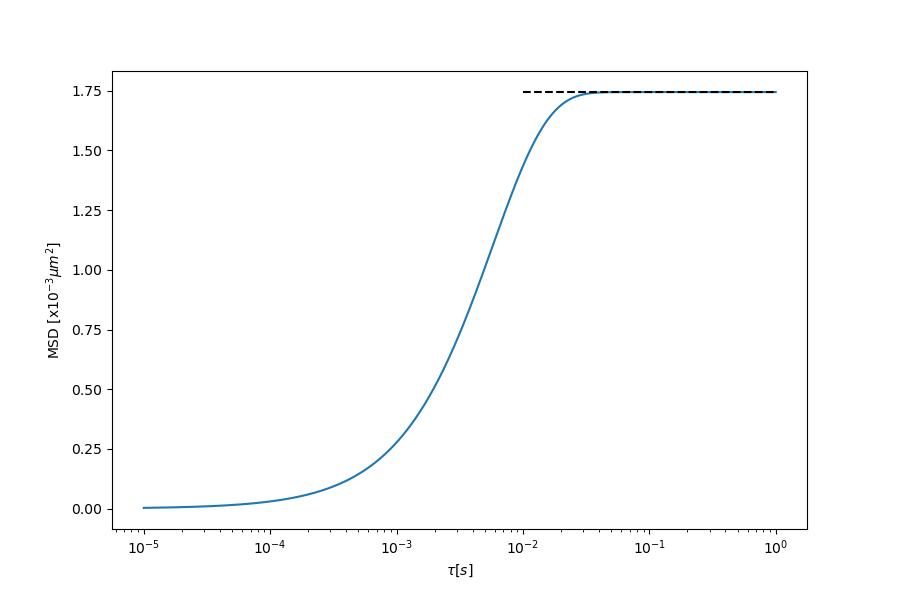
\includegraphics[width=\linewidth]{MSD.png}
	\caption{Example mean squared displacement using \eqref{eq:MSD}, 
		for a $1\mu m$ sphere trapped by an optical potential well. 
		The dotted line represents the upper limit of the sphere's 
		displacement due to the optical trap.}
	\label{fig:MSD}
\end{figure}

The MSD plot can be subdivided into two regimes, when $\tau \gg \tau_{OT}$ 
the particle is experiencing the harmonic potential described by 
the equipartition theorem, and when $\tau \ll \tau_{OT}$ the particle 
is said to be freely diffusing within the trap focus. Of course for 
a freely diffusing object the MSD will never reach a plateau value, 
comparing MSD's for different particles provides a simple visual 
indicator of the difference in trapping strength. The MSD method is 
an already very versatile analytical tool for diffusive motion, however 
it is rather slow in computing time meaning it is only really beneficial 
when a high degree of accuracy is required and shorter time resolutions 
are unavailable - such as using a quadrant photo diode instead or a high 
speed CCD.

\subsubsection{Mean Square Angular Displacement (MSAD)}
It is also possible to plot the angular MSD (MSAD) using 
simulative or experimental data, but there is no complementary 
expression for Eq.~\eqref{eq:MSD}. This is because while the 
particle is close to the focus the optical force is easily 
modelled as a Hookean spring, even if the particle undergoes
some rotation. Conversely, the optical torque applied to a 
particle is far more sensitive to changes in position meaning 
a simple linear approximation is not satisfactory. 
Vigilante \textit{et al} \cite{Vigilante2020} derived the 
upper limit of a dimer's MSAD along its long axis by assuming 
it was strongly trapped and so had limited angular motion, 
there expression gives:
\begin{align}
	\lim_{\tau\to\infty}\left<(\Delta u_z)^2\right> = 
	2\left[1-\frac{1}{4\beta\kappa_r} 
	\left(\frac{exp(\beta\kappa_r)-1}
	{exp(\beta\kappa_r)F(\sqrt{\beta\kappa_r})
	}\right)^2\right]
\end{align}  

Where, $u_z$ is the unit vector connecting the two spheres of 
the dimer, $\beta=1/k_BT$, $\kappa_r$ is the rotational stiffness 
of the trap, and $F$ is Dawson's integral \cite{Oldham2008}. 
Vigilante's paper expressed that they couldn't compute 
$MSAD(\tau)$ because they couldn't solve the Einstein-Smoluchowski 
equation which describes the diffusion constant for dielectric 
particles. This would require a full description of a particle's 
electrical mobility and charge distribution - the latter could be 
achieved via a discrete dipole approximation, the former would be 
dependent on both the particle's position and relative orientation 
to the electric field.

\subsection{Power Spectrum Density (PSD)}
The power spectral density (PSD) method is by far the most versatile 
method for observing the dynamics of any object within an optical trap, 
allowing for fast calibration times while also quickly filtering out 
typical noise sources. After recording a trajectory over some time 
$t_{msr}$, taking the Fourier transform of a particle's trajectory 
yields:
\begin{align}
	\hat{x}(f) = \frac{(2D)^{1/2}\hat{\eta}}{2\pi(f_c-if)}
\end{align}

where $x$ can either be the physical position (relative to the trap
focus) or a recorded signal from a position-detector, and $\hat{\eta}$ 
is the Fourier transform of the white noise (see Eq.~\eqref{eq:full_langevin}). Where the values are exponentially distributed as opposed to being normally distributed in the time 
domain \cite{BergSoerensen2004}. We can therefore ignore the white 
noise from our analysis by looking at the spectral density of $\hat{x}(f)$ that produces a Lorentzian
curve: 
\begin{align}
	\label{eq:lorentzian}
	S_x = \frac{\hat{x}^2}{t_{msr}} = \frac{D}{2\pi(f_c^2+f^2)}
\end{align}
 
Eq.~\eqref{eq:lorentzian} can be fitted via a simplified geometric 
series $S_x = 1/(A+Bf_k^2)$ which allows us to compute both the 
diffusion coefficient (in arbitrary units) and the corner frequency 
$f_c$ which is directly related to the trap strength via $f_c = 
\kappa_x/(2\pi\gamma)$. The Lorentzian shape implies that the trap 
is harmonic - but not symmetric - which assumes that the particle 
itself is an isotropic scatterer. Anisotropic scatterers can 
produce an Lorentzian curve if the angular component of the power
spectra is insignificant. The magnitude of rotational motion 
(whether it is stochastic \cite{Bang2020} or periodic 
\cite{Yogesha2012}) will effect how drastically it departs from a 
typical Lorentzian curve.

Like with the analytical expression of the mean squared displacement we 
see two distinct regions, when $f\ll f_c$ the PSD reaches a plateau value 
that when converted to length units represents the maximum displacement 
the particle can move beyond the focus. When $f\gg f_c$ the PSD falls 
off exponentially which denotes the particle is freely diffusing within 
the beam focus.
\begin{figure}[h!]
	\centering
	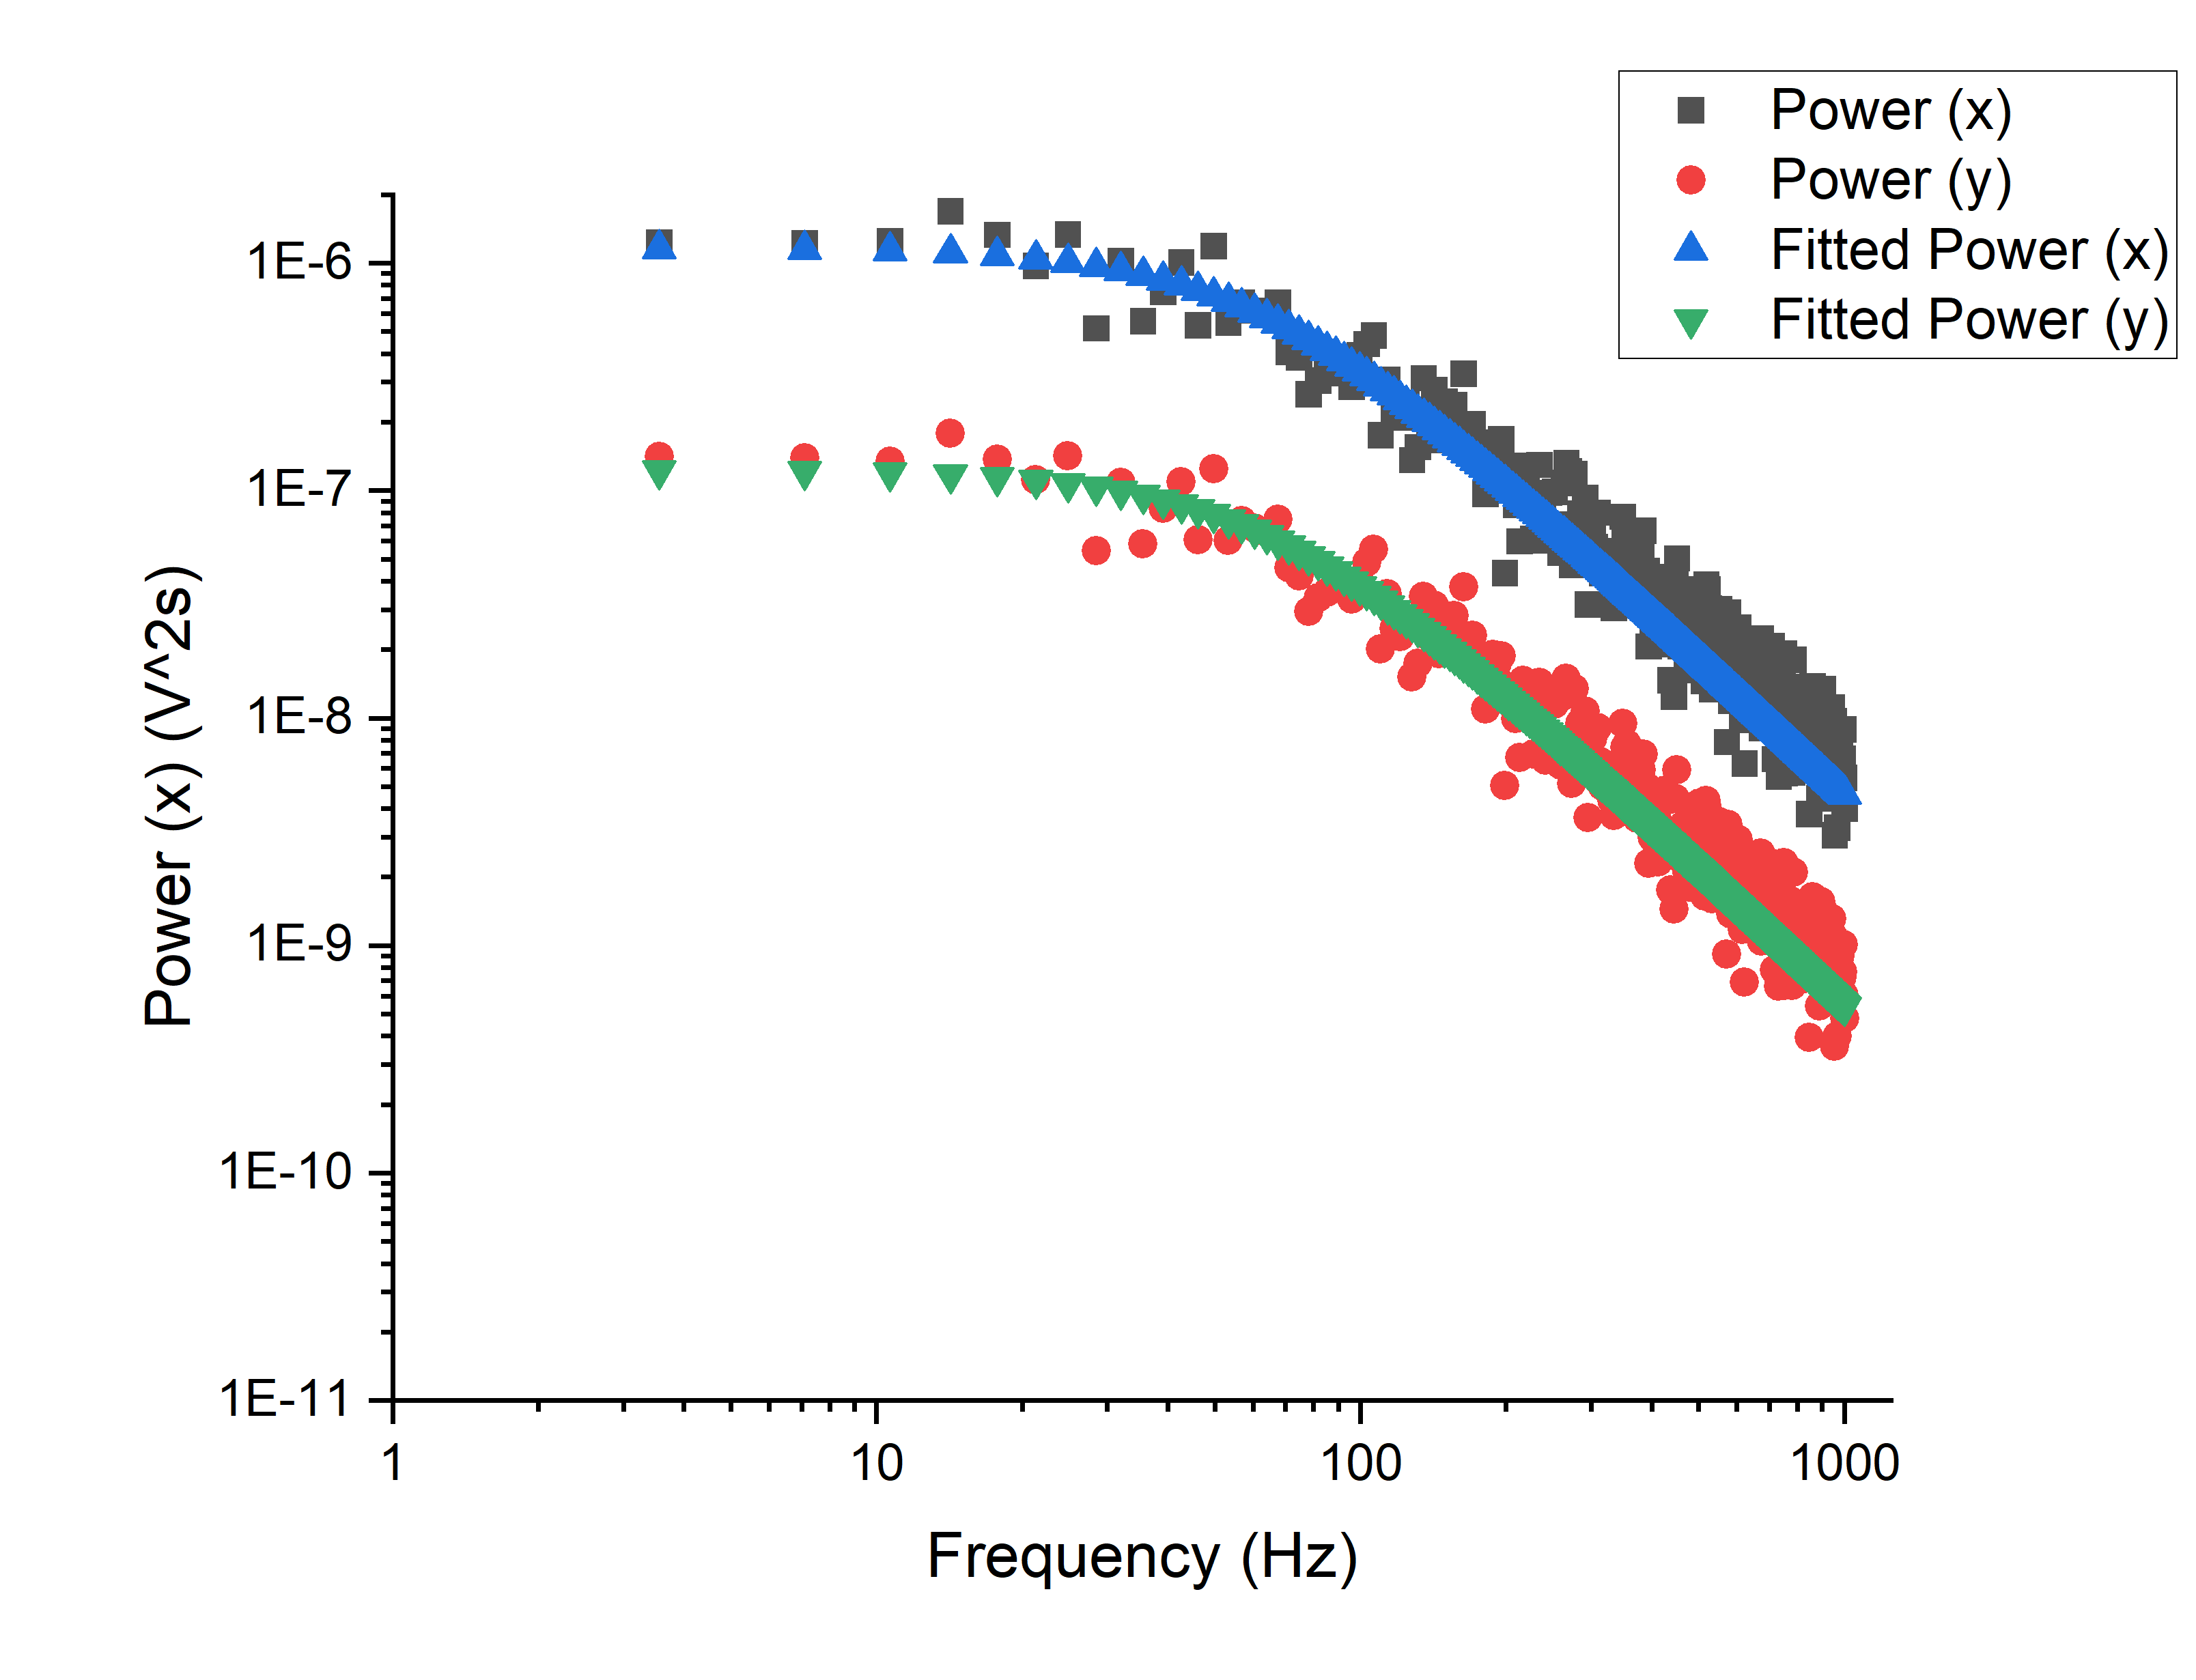
\includegraphics[width=\linewidth]{PSD.png}
	\caption{Example PSD fitted using \eqref{eq:lorentzian}, power 
		spectra is collected from an optically trapped silica sphere 
		suspended in water. The difference in magnitude is due to 
		the asymmetry of the quadrant photo diode having a stronger 
		signal response in the direction of the polarisation vector. 
		Using a conversion factor (see \eqref{eq:conversion_factor}) 
		will adjust the power spectra to better describe the trap shape.}
\end{figure}

The Lorentzian relationship is only valid for frequency terms up to 
the Nyquist frequency (half of our sampling rate), this is because we 
are only taking a finite sampling of the particle's trajectory meaning 
the signal is aliased. Berg and Sorensen provide a suitable modified 
Lorentzian to account for the aliasing effects \cite{BergSoerensen2004}:
\begin{align}
	\label{eq:alaised_lorentzian}
	S_x = \frac{(\Delta x)^2\Delta t}{1+c^2-2c\cos{2\pi f_k\Delta t/N}}
\end{align}

Where N is the total number of samples taken, $\Delta x \ \& \ c$ 
have no direct physical interpretation and are defined in 
\cite{BergSoerensen2004}. Further modifications can be made to the 
power spectrum model but this is only useful when a high degree of 
accuracy is necessary. Typically power spectra are recorded using 
a Quadrant Photo Diode (QPD), which records motion in voltage units, 
not in units of length. There are two main methods for converting to
physical units: If multiple photodetectors are available then a 
differential interference contrast (DIC) system can be used to 
compute the linear relationship between the beads displacement and 
the photodiodes signal \cite{Capitanio2002}. While this is useful 
when high force precision is necessary it also allows you to collect information about the particle's motion along a single direction, 
making it ideal for less focused beams. Alternatively, if the size distribution is very wide but each particle can be accurately sized, 
then a conversion factor can be approximated by comparing the fitted 
value of the diffusion coefficient, and the reported value given by 
the Stokes-Einstein relation.
\begin{align}
	\label{eq:conversion_factor}
	D_{SE} = \frac{k_BT}{\gamma_0} \Rightarrow Conversion\ Factor \ [m/V]= \sqrt{\frac{D_{SE}}{D_{fit}}}
\end{align}

With the latter method, the local fluid viscosity must be known to a 
high degree of accuracy, depending on the local heating effect this 
may be a trivial increase or it may be significant enough to drastically 
alter the characterisation. This also assumes that the particle shape is known, and by implication its diffusion tensor. PSD analysis is often seen as the gold standard for calibration as it can be fine tuned to the point that optical forces can be computed on the order of $10^{-15} N$ 
\cite{BergSoerensen2004}, it captures all of the information acquired 
by other calibration techniques while filtering out noise and requiring 
a relatively small amount of data collection. 

\subsubsection{Power spectral analysis for rotating objects}
The scattering from rotating objects can be partially characterised via
the power spectrum density method. If the particle is birefringent then
as it rotates the detected signal will oscillate periodically. When a 
Fourier transform of the time series is taken the power spectra will 
have a peak signal at that periodic frequency. Typically papers 
reporting on the rotation rate of a trapped object will collect a power spectrum and look at the maximum frequency term to determine its rotation rate. However this often neglects any information on the trapping forces acting on particle and only looks at the torque applying around one of the particle's primary axis. There has only been one notable effort to fully characterise the full trapping dynamics on a rotating body, \cite{Yogesha2012} developed a theoretical model that relates the power spectrum to both the rotational and translational motion simultaneously. This is applicable to particles with a polarizable long axis but is insufficient for birefringent particles.


